% Created 2016-05-02 Mon 16:36
\documentclass[11pt]{article}
\usepackage[latin1]{inputenc}
\usepackage[T1]{fontenc}
\usepackage{fixltx2e}
\usepackage{graphicx}
\usepackage{longtable}
\usepackage{float}
\usepackage{wrapfig}
\usepackage{soul}
\usepackage{textcomp}
\usepackage{marvosym}
\usepackage{wasysym}
\usepackage{latexsym}
\usepackage{amssymb}
\usepackage{hyperref}
\tolerance=1000
\providecommand{\alert}[1]{\textbf{#1}}

\title{Software Architecture Case Study Report for Apache HTTP Server}
\author{Ashwini Tokekar [201405546],Deepak Kathayat [201101213],M.S.Soumya [201450872]}
\date{\today}
\hypersetup{
  pdfkeywords={},
  pdfsubject={},
  pdfcreator={Emacs Org-mode version 7.9.3f}}

\begin{document}

\maketitle

\setcounter{tocdepth}{3}
\tableofcontents
\vspace*{1cm}


\section{INTRODUCTION}
\label{sec-1}
\subsection{History of Apache}
\label{sec-1-1}

   The Apache HTTP server is an open source project which was built
   collaboratively by 8 contributors often known as the core
   contributors. The software development was aimed at creating a robust,
   commercial-grade, and featureful implementation of an HTTP server. Now
   the organization has evolved and has a large number of committers who
   are given access to the source code of the repositories to help
   maintain the project or its relevant docs.  The core group now manages
   the project and is called the Project management Committee (PMC for
   short). The name Apache was chosen as a sign of respect for the native
   American Indian tribe of Apache, well known for their superior skills
   in warfare strategy and inexhaustible endurance. It also makes a cute
   pun on ``a patchy web server'' -- a server made from a series of
   patches. The group of developers who released this new software soon
   started to call themselves the ``Apache Group''.
\subsection{Uses}
\label{sec-1-2}

   The apache web server is used for hosting web sites. 
\section{REQUIREMENTS AND QUALITIES}
\label{sec-2}
\subsection{Feature overview}
\label{sec-2-1}

Apache supports a variety of features, many implementations compiled
as modules that extends the basic functions. These can range from
support for server-side authentication system programming
language. Some common language interfaces support Perl, Python, Tcl,
and PHP. Modules include popular approval mod$_{\mathrm{access}}$, the mod$_{\mathrm{auth}}$,
mod$_{\mathrm{digest}}$ and mod$_{\mathrm{auth}}$$_{\mathrm{digest}}$ successor to mod$_{\mathrm{digest}}$. Other features
examples include Secure Socket Layer and Transport Layer Security
support (mod$_{\mathrm{ssl}}$), the proxy module (mod$_{\mathrm{proxy}}$), the unit re-write the
title (mod$_{\mathrm{rewrite}}$), the special log file (mod$_{\mathrm{log}}$$_{\mathrm{config}}$), and
support for the candidate ( mod$_{\mathrm{include}}$ responsible and
mod$_{\mathrm{ext}}$$_{\mathrm{filter}}$).

Some of Apache��s popular compression methods, including external
expansion modules, mod$_{\mathrm{gzip}}$ are implemented to help reduce the size
(weight) of web pages via HTTP. ModSecurity is an open source Web
intrusion detection and prevention of the engine application. Apache
logs can be analysed using free scripts such as AWStats software /
W3Perl or Visitors through a Web browser.

Virtual hosting allows an Apache installation to serve many different
sites. For example, single installation can serve www.example.com,
www.example.org, test47.test-server.example.edu etc. simulateonusly.


Apache has error messages that are configurable, with the
authentication databases formality-based database management systems,
and allows the content negotiation. And also it supports by many of
the graphical user interface (GUI) for.  It supports password
authentication and digital certificate authentication. Since the
source code is free, anyone can be adapt the server to their specific
needs, also there is a library of Apache plug-ins.
\subsection{Functional Requirements}
\label{sec-2-2}

\begin{itemize}
\item URI to filename translation
\item Several phases involved with access control
\item Determining the MIME type of the requested entity
\item Actually sending data back to the
\item Client logging the request.
\end{itemize}
\subsection{Non-Functional Requirements}
\label{sec-2-3}

\begin{itemize}
\item Per-directory configuration
\item Allowing native functionality to be superseded
\item Backward compatibility ensured
\item There must be protocol independence
\end{itemize}
\subsection{Functionalities provided by Apache HTTP server}
\label{sec-2-4}

HTTP server and proxy features
Loadable Dynamic Modules
Multiple Request Processing modes (MPMs) including Event-based/Async, Threaded and Prefork.
Highly scalable (easily handles more than 10,000 simultaneous connections)
Handling of static files, index files, auto-indexing and content negotiation
.htaccess support
Reverse proxy with caching
Load balancing with in-band health checks
Multiple load balancing mechanisms
Fault tolerance and Failover with automatic recovery
WebSocket, FastCGI, SCGI, AJP and uWSGI support with caching
Dynamic configuration
TLS/SSL with SNI and OCSP stapling support, via OpenSSL.
Name- and IP address-based virtual servers
IPv6-compatible
HTTP/2 protocol support
Fine-grained authentication and authorization access control
gzip compression and decompression
URL rewriting
Headers and content rewriting
Custom logging with rotation
Concurrent connection limiting
Request processing rate limiting
Bandwidth throttling
Server Side Includes
IP address-based geolocation
User and Session tracking
WebDAV
Supports Embedded Perl, PHP and Lua scripting and CGI 
public$_{\mathrm{html}}$ per-user web-pages
Generic expression parser
Real-time status views
XML support
\section{ARCHITECTURAL SOLUTION}
\label{sec-3}
\subsection{Overview}
\label{sec-3-1}

    Apache HTTP server contains a relatively small core, together with a
    number of units. The units can be statically compiled into the server
    or, more commonly, stored in the / modules / or the \emph{libexec} guide
    maintain and then can be dynamically loaded at runtime.

    In addition, the server relies on the Apache Portable Runtime (APR)
    libraries, which provide a cross-platform operating system layer and
    utilities,so that modules don��t have to rely on non-portable
    operating system calls.In addition, the server depends on the Apache
    Portable Runtime (APR) libraries that provide a cross platform
    operating system layer and utilities, so that the units do not have
    to rely on the operating system calls that are not portable.A module
    for special purposes, the Multi-Processing Module (MPM), is working
    to improve the Apache to the underlying operating system. It must be
    the MPM that usually is the only unit to gain access to another
    operating system through APR.

    \begin{figure}[htb]
    \centering
    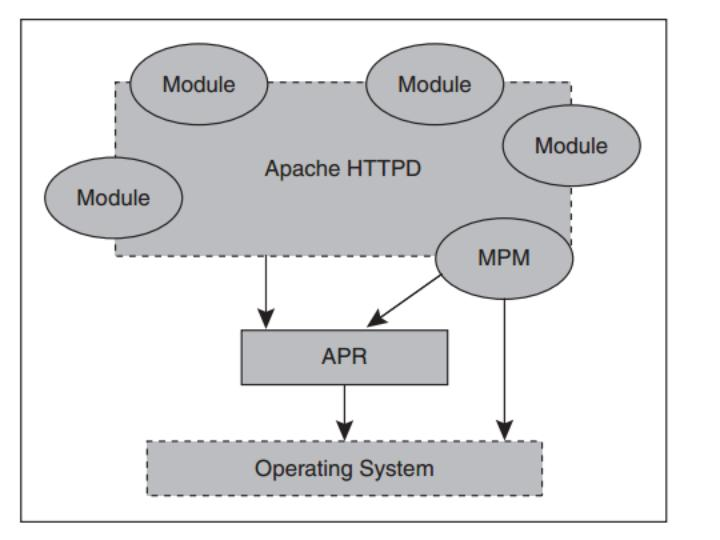
\includegraphics[width=.9\linewidth]{./architecture-overview.jpg}
    \caption{Overview diagram}
    \end{figure}
\subsection{Two-Phase Operation}
\label{sec-3-2}

   Apache Server operates in two stages: start-up and operational. At
   Start-up stage the server is in root mode, and includes analysis of
   the configuration file(s), loading modules, and the instantiation
   of system resources such as log files, shared memory segments, and
   database connections.  In Normal operation, Apache gives up the
   system privileges and works as a normal user before accepting and
   processing connections from clients across the network. This
   two-stage process has some implications for applications
   architecture.

   First, you must run anything that requires system privileges in the
   startup. Second, it's a good practice to run as much as possible
   configuration at startup, to ensure that processing is reduced when
   each request is serviced.On the contrary, because a lot of slow and
   expensive operations are concentrated in the startup stage, it
   would be inefficient to try run the Apache from a generic server,
   such as inetd or tcpserver. A non-trivial aspect of the
   architecture is that the code configuration is, in fact, executed
   twice at startup (although not at the restart).The first time
   through the checks that the configuration is valid (at least to the
   point that can successfully start Apache); the second pass is
   ``live'' and leads to the operational phase. Most units can be ignore
   this behavior (the use of the standard in APR pools ensure that it
   does not cause a resource leak), but may have an impact on some
   units.For example, the unit that holds the new code dynamically
   loads it in the startup phase may want to do this only once, and
   therefore, it must use a technique such as setting and checking of
   a static flag to ensure it��s creation of one-time only.
\subsubsection{Start-up Phase}
\label{sec-3-2-1}

    The purpose of the startup of the Apache is to read the
    configuration, load modules, libraries, and create the necessary
    resources. Each unit may have its own resources, and has an
    opportunity to create those resources. In the startup phase,
    Apache runs as a single process,single-thread program and has root
    privileges.
\begin{itemize}

\item Configuration\\
\label{sec-3-2-1-1}%
The main configuration file in Apache is usually called as
     httpd.conf file. However, this is just a convention, a
     third-party Apache distribution such as those provided as .rpm or
     .deb packages may use different nomenclature.In addition, it may
     be a single file, or may be divided into multiple files using the
     Include guidance to include various configuration files. Some
     distributions have a very complex configurations.For example,
     Debian GNU/Linux Apache configuration, relies heavily on the
     familiarity with Debian, not with Apache. The configuration file
     httpd.conf file is a plain text file which is analysed line by
     line at server startup. The contents of the file include
     directives, containers, and comments. It also allows empty lines
     and leading whitespaces, but will be ignored.

\end{itemize} % ends low level
\subsubsection{Operational Phase}
\label{sec-3-2-2}

    At the end of the start-up stage,the control passes to the
    Multi-Processing Module(MPM). The MPM is responsible for managing
    the Apache functioning on the systems level. It usually does so by
    maintaining a set of worker processes and/or threads, as
    appropriate with the operating system and other applicable
    constraints (such as the optimization for a specific use).The
    original process remains as the ``master'' to maintain a set of
    worker children. These workers are responsible for entertaining
    incoming connections, while the parent process deals with the
    creation of a new children , and the removal of the surplus when
    necessary, and communication signals such as ``shutdown'' or
    ``restart.''Because of the MPM structure, it is not possible to
    describe the operation phase in the definite terms. The standard
    MPMs use the worker children in some manner so that, they are not
    limited only work in one way. Thus, it can be another MPM achieve
    in principle, to implement a completely different system-level
    server architecture.
\subsubsection{Shutdown}
\label{sec-3-2-3}

    There is no shutdown phase as such. Instead, anything that needs
    be done on shutdown is registered as a cleanup. When Apache stops,
    all registered cleanups are run.
\subsection{Multi-Processing Modules}
\label{sec-3-3}

   At the end of the start-up phase, having been read configuration,
   full control of the Apache passes to a Multi-Processing Module. MPM
   acts an interface between the running Apache server and the
   underlying operating system.  Its primary role is to improve the
   Apache platform, while ensuring the server to work efficiently and
   securely. As the name suggests, MPM is in itself a module . But MPM
   is a unique systems level (even the development of MPM is outside
   the scope of a book about the development of applications).  Also
   uniquely, Apache instance contains single MPM, which is determined
   at build-time. An MPM��s responsibilites are located inside the main
   loops of the Apache. The main server does the initialization and
   configuration for processing before calling ap$_{\mathrm{mpm}}$$_{\mathrm{run}}$() function
   in main() to be delivered to MPM.It is the responsibility of the
   MPM to take care of starting the threads and / or processes as
   required. MPM will also be responsible for listening on sockets for
   incoming requests. Upon the arrival of requests, the MPM
   distributes them between the threads and/or processes that have
   been created. And then run the Apache standard procedures for
   request handling. When you restart or shut down, the MPM delivered
   back to the main server.  So,each server functionality is still the
   same for any MPM, but the multi-processing model
   interchangeable. The figure below shows the responsibility of
   Apache MPM in the general behavior of the Apache. The dotted line
   represents the actions of MPM takes responsibility.

   \begin{figure}[htb]
   \centering
   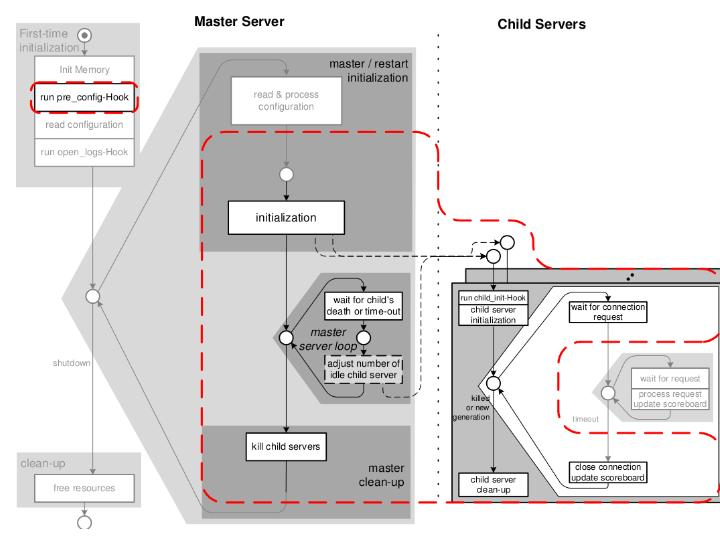
\includegraphics[width=.9\linewidth]{./leader-followers-archiecture.jpg}
   \caption{Responsibility of an Apache 2.0 MPM}
   \end{figure}
\subsection{The leader-followers pattern}
\label{sec-3-4}

  The preforking structure is based on a set of tasks (processes or
  threads) that play three different roles:
\begin{itemize}
\item Wait for requests (the listener)
\item Request processing (worker)
\item Queue in wait to become a listener (idle worker)
\end{itemize}

  \begin{figure}[htb]
  \centering
  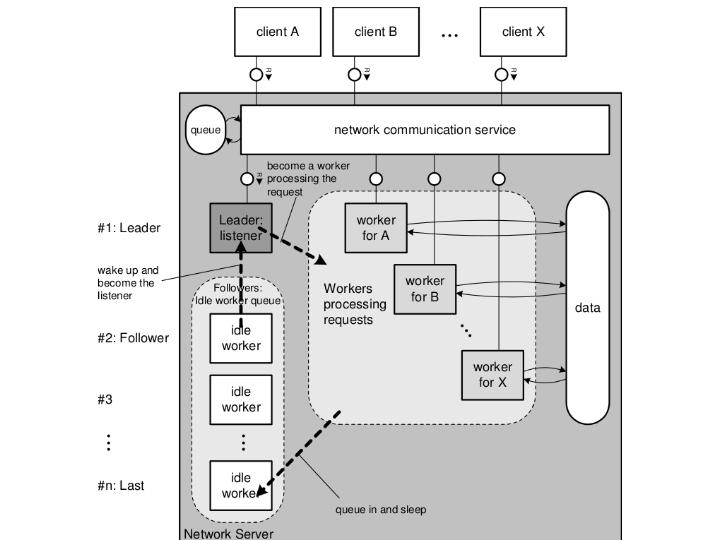
\includegraphics[width=.9\linewidth]{./fig-3.jpg}
  \caption{The leader-followers pattern used in the preforking server architecture}
  \end{figure}
  Listener is the leader.The right to wait for connection requests can
  be granted to only one task. If listener gets a request, it provides
  the right to listen, he switches the role to worker, which implies
  that it processes the request using the connection established as
  listener. If it is done processing the request, it will close the
  connection becomes idle worker. This means that it queues in waiting
  to become the listener. Usually an idle worker task will be
  suspended.  
\subsection{Preforking Architecture}
\label{sec-3-5}


  The the first multi-tasking architecture of Apache was Preforking
  Architecture. In Apache 2.0, which is still the default MPM for
  Unix. The Netware MPM is very similar to the Apache Preforking
  except that it uses Netware threads instead of Unix processes.

  Summarizing, the Apache Preforking Architecture takes the
  traditional approach where each child server is a process in
  itself. This makes Preforking stable architecture but also reduces
  performance. The following figure shows how the Apache Web Server
  provides a powerful multi-processing module, which is based on
  preforking process, Apache-MPM prefork.


  \begin{figure}[htb]
  \centering
  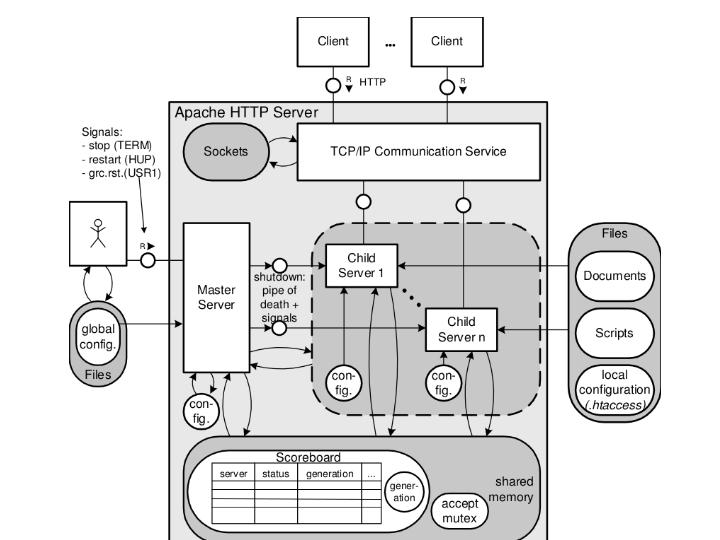
\includegraphics[width=.9\linewidth]{./preforking.jpg}
  \caption{The Apache 2.0 Preforking MPM}
  \end{figure}


  The following figure shows the overall behavior of the server,
  including the master server and the child servers.
  
  \begin{figure}[htb]
  \centering
  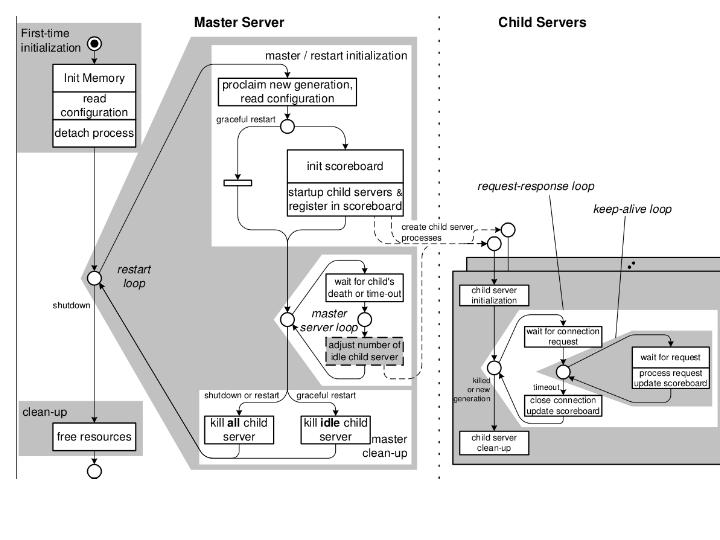
\includegraphics[width=.9\linewidth]{./apache-behaviour.jpg}
  \caption{Overview: The behavior of Apache}
  \end{figure}

  Independent of the multitasking architecture, Apache��s behavior
  consists of the sequence of following parts that will be discussed
  individually for each of the architecture:
\begin{description}
\item[The first time initialization] Resource allocation, and read and review configuration, become
       a daemon.
\item[The restart loop] Re-read configuration, create task pool gathered from the child
       server processes and enter the main server loop.
\item[The main server loop] To control the number of idle child server processes in the job
       pool.
\item[Respond to a request loop (only child server)] Wait to become a leader, and wait for a connection request,
       become a worker and enter the keep-alive loop.
\item[The keep-alive-loop(only child server)] 
\begin{itemize}
\item Handle HTTP requests
\item Cleaning master server and child servers before deactivation
\end{itemize}
\end{description}
\section{REFERENCES}
\label{sec-4}

\begin{thebibliography}{20}

\bibitem{open-source-architecture-book}
Amy Brown and Greg Wilson.
\emph{The Architecture of Open Source Application- Elegance, Evolution, and a Few Fearless Hacks},

\bibitem{apache-org}
\emph{https://httpd.apache.org/ABOUT_APACHE.html}.

\bibitem{server-architecture}
\emph{http://berb.github.io/diploma-thesis/original/042_serverarch.html}.

\bibitem{multi-tasking}
\emph{http://www.fmc-modeling.org/category/projects/apache/amp/4_3Multitasking_server.html#sub:Overview-Apache-Multitasking-Arch}.

\bibitem{apache-platform-arch}
\emph{http://ptgmedia.pearsoncmg.com/images/9780132409674/samplechapter/kew_ch02.pdf}.

\bibitem{intro-apache-web-server}
\emph{http://apachecon.com/2007/notes/t02-notes.pdf}.

\bibitem{apache-design}
\emph{http://iw3c2.cs.ust.hk/WWW5/www5conf.inria.fr/fich_html/papers/P20/Overview.html}.

\bibitem{apache-project}
\emph{http://ieeexplore.ieee.org/stamp/stamp.jsp?tp=&arnumber=612229}.

\end{thebibliography}
\section{EFFORT}
\label{sec-5}



\begin{center}
\begin{tabular}{ll}
\hline
 Name     &  Time spent  \\
\hline
 Ashwini  &  7 hrs       \\
 Deepak   &  7 hrs       \\
 Soumya   &  7 hrs       \\
\hline
\end{tabular}
\end{center}

\end{document}
